%% Based on a TeXnicCenter-Template by Gyorgy SZEIDL.
%%%%%%%%%%%%%%%%%%%%%%%%%%%%%%%%%%%%%%%%%%%%%%%%%%%%%%%%%%%%%

%----------------------------------------------------------
% title
%		\title[This is my Title]{Presentation\\ Title}	
	% author 
    % (In the mandatory argument "{}", separate multiple
    % authors with "\and" - use "\\" for better author name formatting
    % in the title page. In the optional argument "[]" include all
	% author names, with no "\and" or text formatting macros.)
	% Example: 
    %\author[A. Author Albert Einstein]{Anthony Author \and Albert Einstein}
		%\author[A. Author]{Anthony Author}
	% supervisor	
		%\supervisor{Supervisor}{Mister Supervisor}{Professor}
	% date
		%\presentationDate{October 22, 2017}
%
\documentclass[spanish,a4paper]{beamer}%
\usetheme{Berlin}%Berlin}Luebeck
%% CUSTOM COLOR
%\definecolor{myyellow}{rgb}{.9,.9,.1}
%\usecolortheme[named=myyellow]{structure}
\usecolortheme{whale}

\makeatletter
\let\beamer@writeslidentry@miniframeson=\beamer@writeslidentry%
\def\beamer@writeslidentry@miniframesoff{%
  \expandafter\beamer@ifempty\expandafter{\beamer@framestartpage}{}% does not happen normally
  {%else
    % removed \addtocontents commands
    \clearpage\beamer@notesactions%
  }
}
\newcommand*{\miniframeson}{\let\beamer@writeslidentry=\beamer@writeslidentry@miniframeson}
\newcommand*{\miniframesoff}{\let\beamer@writeslidentry=\beamer@writeslidentry@miniframesoff}

\setbeamertemplate{headline}
{%
  \begin{beamercolorbox}[colsep=1.5pt]{upper separation line head}
  \end{beamercolorbox}
  \begin{beamercolorbox}{section in head/foot}
    \vskip2pt\insertsectionnavigationhorizontal{\paperwidth}{}{}\vskip2pt
  \end{beamercolorbox}%
  \ifbeamer@theme@subsection%
    \begin{beamercolorbox}[colsep=1.5pt]{middle separation line head}
    \end{beamercolorbox}
    \begin{beamercolorbox}[ht=2.5ex,dp=1.125ex,%
      leftskip=.3cm,rightskip=.3cm plus1fil]{subsection in head/foot}
      \usebeamerfont{subsection in head/foot}\insertsubsectionhead
    \end{beamercolorbox}%
  \fi%
  \begin{beamercolorbox}[colsep=1.5pt]{lower separation line head}
  \end{beamercolorbox}
}
\makeatother
\setbeamerfont{block body}{size=\small}
%\setbeamertemplate{footline}[page number] 

\usepackage[spanish, es-tabla]{babel}
\usepackage{float}
\usepackage[utf8]{inputenc}
\usepackage{color}
\usepackage{amsmath}
\usepackage{amsfonts}
\usepackage{amssymb}
\usepackage{cite}
\usepackage{epstopdf}
\usepackage{array}
\usepackage{multirow}
\usepackage{multicol}
\sloppy
\epstopdfsetup{outdir=./pdf}
\usepackage{graphicx}

\usepackage{caption}
\usepackage{subcaption}
\usepackage{nameref}
\makeatletter
\newcommand*{\currentname}{\@currentlabelname}
\makeatother
%\usepackage{etoc}
%para generar índice con hipervínculos
\usepackage{hyperref}


%parametros del documento (sus propiedades)
\hypersetup{
    pdftitle={Martin Augusto Reigadas Teran - TFG - 2022},
    pdfsubject={TFG - 2022},
    pdfauthor={Martin Augusto Reigadas Teran},
    pdfkeywords={termo-fotovoltaica} {campo cercano} {recuperación de calor},
    colorlinks,
    citecolor=black,
    filecolor=black,
    linkcolor=black,
    urlcolor=black,
}

\title[\color{white} \tiny Modelado y simulación de espaciadores nanométricos para su aplicación en dispositivos TPVs de campo cercano]{\LARGE Modelado y simulación de espaciadores nanométricos para su aplicación en dispositivos TPVs de campo cercano}
\author[Martin Augusto Reigadas Teran]{\large Martin Augusto Reigadas Teran}
\institute{Universidad Politécnica de Madrid}
%\supervisor{Tutor}{Pablo García-Linares Fontes}{Profesor}
\date{Septiembre, 2022}

%\AtBeginSection[]{
%\begin{frame}{Tabla de Contenidos}
%	\tableofcontents[currentsection,hideallsubsections]
%\end{frame}
%}
\AtBeginSection[]
{
   \begin{frame}<beamer>{\currentname}
        \tableofcontents[currentsection,currentsubsection,hideallsubsections, 
    sectionstyle=show/shaded,subsectionstyle=show/shaded/hide]
   \end{frame}
}
\AtBeginSubsection[]
{
   \begin{frame}<beamer>{\currentname}
        \tableofcontents[currentsubsection,hideothersubsections,hideothersubsections, 
    sectionstyle=hide,subsectionstyle=show/shaded]
   \end{frame}
}
\begin{document}
\graphicspath{{./figuras/}}
	%\metroset{block=fill}

	%% TITLE PAGE
	{
		\setbeamercolor{author in head/foot}{use=palette secondary, fg=palette secondary.bg} 
		\setbeamercolor{institute in head/foot}{use=palette secondary, fg=palette secondary.bg}
		\setbeamercolor{section in head/foot}{use=palette tertiary, fg=palette tertiary.bg}
		\setbeamercolor{subsection in head/foot}{use=palette secondary, fg=palette secondary.bg} 

		\begin{frame}
			\titlepage
			\begin{minipage}[l]{0.48\textwidth}
			\begin{flushleft}
				\footnotesize \itshape  Tutor: Pablo García-Linares Fontes\\
				\tiny Departamento de Ingeniería Eléctrica, Electrónica, Automática y
		Física Aplicada		
			\end{flushleft}
			\end{minipage}\hfill
			\begin{minipage}[r]{0.48\textwidth}
			\begin{flushright}
				\footnotesize \itshape Cotutora: Esther López Estrada\\
				 \tiny Instituto de Energía Solar\\
				
						
			\end{flushright}
			\end{minipage}
		\end{frame}
	}

	%%  TABLA DE CONTENIDOS
	{
		\setbeamercolor{section in head/foot}{use=palette tertiary, fg=palette tertiary.bg}
		\begin{frame}{Tabla de Contenidos}
				\tableofcontents[hideallsubsections]
		\end{frame}
	}

	%% INTRODUCCION
	\section{Introducción}
	\begin{frame}{Introducción}
	
	

	
\only<2->{\begin{columns}}
	\centering
	\only<2->{\column{.5\textwidth}}
			\only<1->{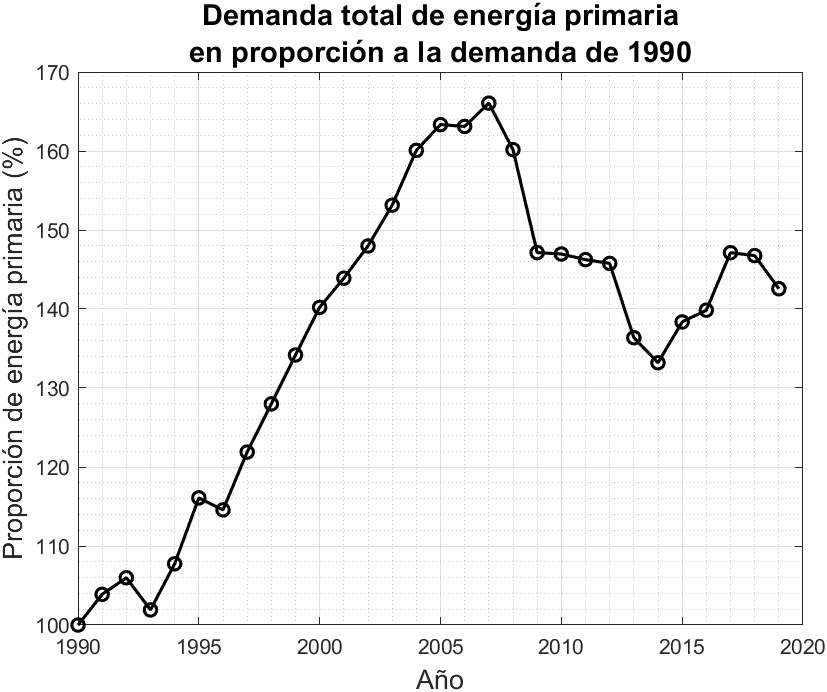
\includegraphics[width=0.6\textwidth]{DemandaEnergiaPrimariaProporcion1990.png}}
		\only<2->{
			%\column{.5\textwidth} 
			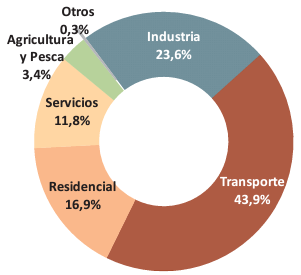
\includegraphics[width=0.4\textwidth]{consumoEnergiaFinalPorSectores_2019.png}}		
			\only<3->{
			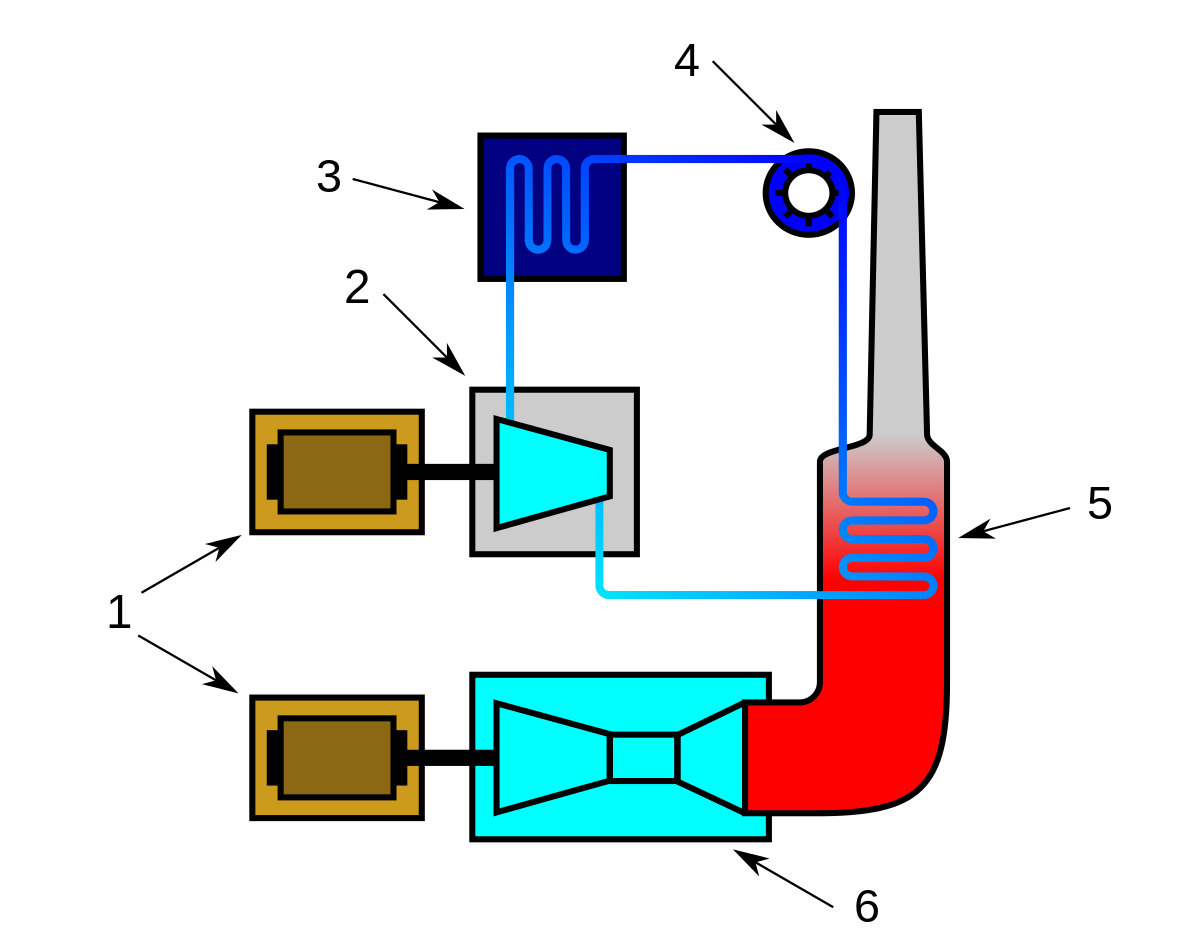
\includegraphics[width=0.50\textwidth]{cicloCombinado.png}}
 \only<2->{\end{columns}}


	\end{frame}

%%  ESTADO DEL ARTE 
	\section{Estado del arte}
	\begin{frame}{Estado del arte}
		
	\end{frame}

%%  MATERIALES Y HERRAMIENTAS
	\section{Materiales y herramientas}
	\begin{frame}{Materiales y herramientas}
		
	\end{frame}


%% METODOS
	\section{Métodos}
	\begin{frame}{Métodos}
		
	\end{frame}

%% RESULTADOS Y DISCUSIÓN
	\section{Resultados y discusión}
	\begin{frame}{Resultados y discusión}
	%\localtableofcontents
		
	\end{frame}
	\subsection{nTPV Si-SiO2-Si}
\begin{frame}{nTPV Si-SiO2-Si}

		
	\end{frame}
		\subsection{nTPV Si-SiO2-Ge}
\begin{frame}{nTPV Si-SiO2-Ge}

		
	\end{frame}
%% CONCLUSIONES
	\section{Conclusiones}
	\begin{frame}{Conclusiones}
	\end{frame}
	\begin{frame}{Desarrollos a futuro}
		
	\end{frame}
%% FINAL
	\miniframesoff
	\section{}
	\begin{frame}	

	\end{frame}

\end{document}
